\documentclass[10pt]{article}

% Idioma y codificación
\usepackage[utf8]{inputenc}
\usepackage[spanish]{babel}

% Márgenes
\usepackage{geometry}
\geometry{top=2.5cm, bottom=2.5cm, left=2.5cm, right=2.5cm}

% Gráficos y Tablas
\usepackage{pdflscape}
\usepackage{graphicx}
\usepackage{pdfpages}
\usepackage{multicol}
\usepackage{float}
\usepackage[table]{xcolor} % UNA SOLA VEZ Y CON [table]
\usepackage{booktabs}
\usepackage{xltabular}
\usepackage{caption}
\usepackage{subcaption}

% Listings para código
\usepackage{listings}
\lstdefinestyle{terminal}{
	backgroundcolor=\color{gray!10},
	basicstyle=\ttfamily\small,
	keywordstyle=\color{blue},
	commentstyle=\color{gray},
	frame=single,
	columns=fullflexible,
	morecomment=[l]{//}
}
\lstset{
	inputencoding=utf8,
	extendedchars=true,
	literate={á}{{\'a}}1 {é}{{\'e}}1 {í}{{\'i}}1 {ó}{{\'o}}1 {ú}{{\'u}}1 {ñ}{{\~n}}1
}

% Hipervínculos
\usepackage[hidelinks]{hyperref}
\hypersetup{
	colorlinks=true,
	linkcolor=blue,
	filecolor=magenta,
	urlcolor=cyan,
}

% Encabezados y pies de página
\usepackage{fancyhdr}
\pagestyle{fancy}
\fancyhf{}
\fancyfoot[R]{\thepage}

% Formato de títulos
\usepackage{titlesec}
\titleformat{\subsection}{\normalfont\large\bfseries}{\thesubsection}{1em}{}
\titleformat{\subsubsection}{\normalfont\normalsize\bfseries}{\thesubsubsection}{1em}{}

% Datos de la portada
\title{\textit{CARD PARTNER}\\ Una web para amantes de los \textit{TCGS}}

\author{
	\textbf{\small ÁLVAREZ FULCONIS, MARCOS PALATINO}\\
	\textbf{\small LÓPEZ PRIMO, ÁLVARO}\\
	\textbf{\small OTERO GARCÍA, SERGIO}\\
	\textbf{\small SANTIESTEBAN MENDO, EDGAR}
}

\date{Curso 25-26}

\begin{document}
	
	\begin{titlepage}
		\centering
		% Asegúrate de que la ruta al PDF de la UVA sea correcta
		%
\includegraphics[scale=0.3]{./Recursos/UVA-3881270087.pdf}\\[0.5cm] 
		\rule{\linewidth}{0.2mm}\\[0.4cm]
		{\huge\bfseries CARD PARTNER\par}
		{\large Una web para amantes de los TCGS\par}
		\rule{\linewidth}{0.2mm}\\[1.5cm]
		{\Large\bfseries Servicios y Sistemas Web}\\[0.3cm]
		{\large\bfseries Laboratorio L2 \\ GRUPO 33}\\[1cm]
		{\Large \begin{tabular}{c} ÁLVAREZ FULCONIS, MARCOS \\ LÓPEZ PRIMO, ÁLVARO \\ OTERO GARCÍA, SERGIO \\ SANTIESTEBAN MENDO, EDGAR \end{tabular}}\\[1.5cm]
		{\Large Curso 25-26}
	\end{titlepage}
	
	\pagenumbering{gobble}
	\tableofcontents \newpage
	
	\pagenumbering{arabic} 
	\setcounter{page}{1}
	
	\section{Especificación de requisitos}
		\subsection{Requisitos funcionales}
		
			\noindent
			\begin{xltabular}{\textwidth}{|l|l|X|}
				\hline
				\rowcolor{gray!20} \textbf{ID} & \textbf{Nombre} & \textbf{Descripción} \\ \hline
				
				\multicolumn{3}{|c|}{\cellcolor{gray!10}\textbf{1. Gestión de Usuarios y Perfiles}} \\ \hline
				RF-1.1 & Registro & Crear cuenta con email y contraseña.  O con una cuenta de Google\\ \hline
				RF-1.2 & Login & Acceso seguro a funciones personalizadas. \\ \hline
				RF-1.3 & Credenciales & Opción de cambio de contraseña desde el perfil y el menú de \textit{login}. \\ \hline
				RF-1.4 & Perfil & Panel central para gestionar datos y activos (en este caso los mazos). \\ \hline
				
				\multicolumn{3}{|c|}{\cellcolor{gray!10}\textbf{2. Gestión y Creación de Mazos}} \\ \hline
				RF-2.1 & Deckbuilder & Herramienta interactiva de selección de cartas. \\ \hline
				RF-2.2 & Almacenamiento & Guardado de mazos en sección privada "Mazos guardados". \\ \hline
				RF-2.3 & Publicación & Compartir mazos con la comunidad. \\ \hline
				RF-2.4 & Biblioteca &  Mostrar los mazos guardados y los propios creados por el usuario \\ \hline
				RF-2.5 & Filtro Comunidad & Búsqueda por Líder. \\ \hline
				RF-2.6 & Estadísticas & Visualización de datos de rendimiento (Meta). \\ \hline
				
				\multicolumn{3}{|c|}{\cellcolor{gray!10}\textbf{3. Base de Datos de Cartas}} \\ \hline
				RF-3.1 & Catálogo & Vista general de todas las cartas del juego. \\ \hline
				RF-3.2 & Filtro Avanzado & Búsqueda por nombre,expansión, color o rareza. \\ \hline
				RF-3.3 & Precios & Mostrar coste de mercado de cartas. \\ \hline
				
				\multicolumn{3}{|c|}{\cellcolor{gray!10}\textbf{4. Comunidad e Interacción}} \\ \hline
				RF-4.1 & Comentarios & Opiniones en mazos de otros usuarios. \\ \hline
				RF-4.2 & Valoración & Sistema de puntuación para destacar mazos (en forma de estrellas de valoración). \\ \hline
				RF-4.3 & Noticias & Sección de novedades y expansiones. \\ \hline
				RF-4.4 & Torneos & Listado de eventos competitivos, con enlaces directos a los resultados. \\ \hline
				
				\multicolumn{3}{|c|}{\cellcolor{gray!10}\textbf{5. Recursos para Principiantes}} \\ \hline
				RF-5.1 & Guía Básica & Explicación de reglas y mecánicas. \\ \hline
				RF-5.2 & Recomendados & Sugerencia de mazos para los mismos. \\ \hline
				
				\multicolumn{3}{|c|}{\cellcolor{gray!10}\textbf{6. Administración y Configuración}} \\ \hline
				RF-6.1 & Admin Panel & Gestión de noticias, torneos y contenidos. \\ \hline
				RF-6.2 & Idioma & Selector de idioma para la interfaz. \\ \hline
				
			\end{xltabular}
			
		\newpage
		\subsection{Requisitos no funcionales}
			
			\noindent
			\begin{xltabular}{\textwidth}{|l|l|X|}
				\hline
				\rowcolor{gray!20} \textbf{ID} & \textbf{Nombre} & \textbf{Descripción} \\ \hline
				
				\multicolumn{3}{|c|}{\cellcolor{gray!10}\textbf{1. Rendimiento y Eficiencia}} \\ \hline
				RNF-1.1 & Tiempo de respuesta & Carga de página principal $<$ 2s y búsquedas $<$ 1,5s. \\ \hline
				RNF-1.2 & Escalabilidad & Soporte de al menos 500 usuarios simultáneos sin degradación. \\ \hline
				RNF-1.3 & Optimización & Uso de formato WebP para imágenes de cartas para reducir ancho de banda. \\ \hline
				
				\multicolumn{3}{|c|}{\cellcolor{gray!10}\textbf{2. Usabilidad y UX}} \\ \hline
				RNF-2.1 & Diseño Responsivo & Funcionalidad total en móviles, tablets y escritorio. \\ \hline
				RNF-2.2 & Aprendizaje & Interfaz del Deckbuilder intuitiva (creación de mazo < 5 min). \\ \hline
				RNF-2.3 & Estética & Diseño coherente con los  bocetos de Práctica 1. \\ \hline
				
				\multicolumn{3}{|c|}{\cellcolor{gray!10}\textbf{3. Seguridad y Privacidad}} \\ \hline
				RNF-3.1 & Protección de datos & Cifrado (hashing) seguro para el almacenamiento de contraseñas. \\ \hline
				RNF-3.2 & Navegación & Implementación de protocolo HTTPS en todo el sitio. \\ \hline
				RNF-3.3 & Validación & Protección contra ataques SQL Injection y XSS en formularios. \\ \hline
				
				\multicolumn{3}{|c|}{\cellcolor{gray!10}\textbf{4. Disponibilidad y Mantenibilidad}} \\ \hline
				RNF-4.1 & Disponibilidad & Tiempo de actividad (\textit{uptime}) garantizado del 90\%. \\ \hline
				RNF-4.2 & Actualización & Inserción de nuevas colecciones sin modificar el código fuente. \\ \hline
				RNF-4.3 & Modularidad & Arquitectura preparada para añadir otros TCG sin reescribir el núcleo. \\ \hline
				
				\multicolumn{3}{|c|}{\cellcolor{gray!10}\textbf{5. Compatibilidad y Portabilidad}} \\ \hline
				RNF-5.1 & Navegadores & Soporte para versiones actuales de Chrome, Firefox, Safari y Edge. \\ \hline
				RNF-5.2 & Estándares & Cumplimiento estricto de estándares W3C (HTML5 y CSS3). \\ \hline
				
			\end{xltabular}
			
	
	\section{Modelo del dominio}
	En esta sección se detalla el modelo conceptual de la aplicación Card Partner, identificando las entidades principales (clases), sus atributos y las relaciones establecidas entre ellas para dar soporte a la lógica del Trading Card Game (TCG) y a la interacción de la comunidad.
	
	Las entidades principales son:
	\begin{itemize}
	    \item \textbf{Usuario:} Clase base de la que heredan \textit{Jugador} y \textit{Administrador}. Contiene la información de autenticación y perfil.
	    \item \textbf{Carta:} Representa la unidad fundamental del juego. Utiliza enumeraciones estrictas para el \textit{Tipo} (Líder, Personaje, Evento, Escenario) y \textit{Color} según las reglas del juego.
	    \item \textbf{Mazo:} Colección de cartas creada por un jugador. Está estrictamente vinculada a una carta \textit{Líder} (relación 1 a muchos) e incluye múltiples cartas en distintas cantidades mediante la clase asociación \textit{Contiene}.
	    \item \textbf{Torneo y Artículos:} Entidades para la gestión de la comunidad, torneos y noticias del juego.
	\end{itemize}

	\begin{figure}[H]
		\centering
		% --- DESCOMENTAR LA SIGUIENTE LÍNEA Y PONER LA RUTA DE VUESTRA IMAGEN ---
		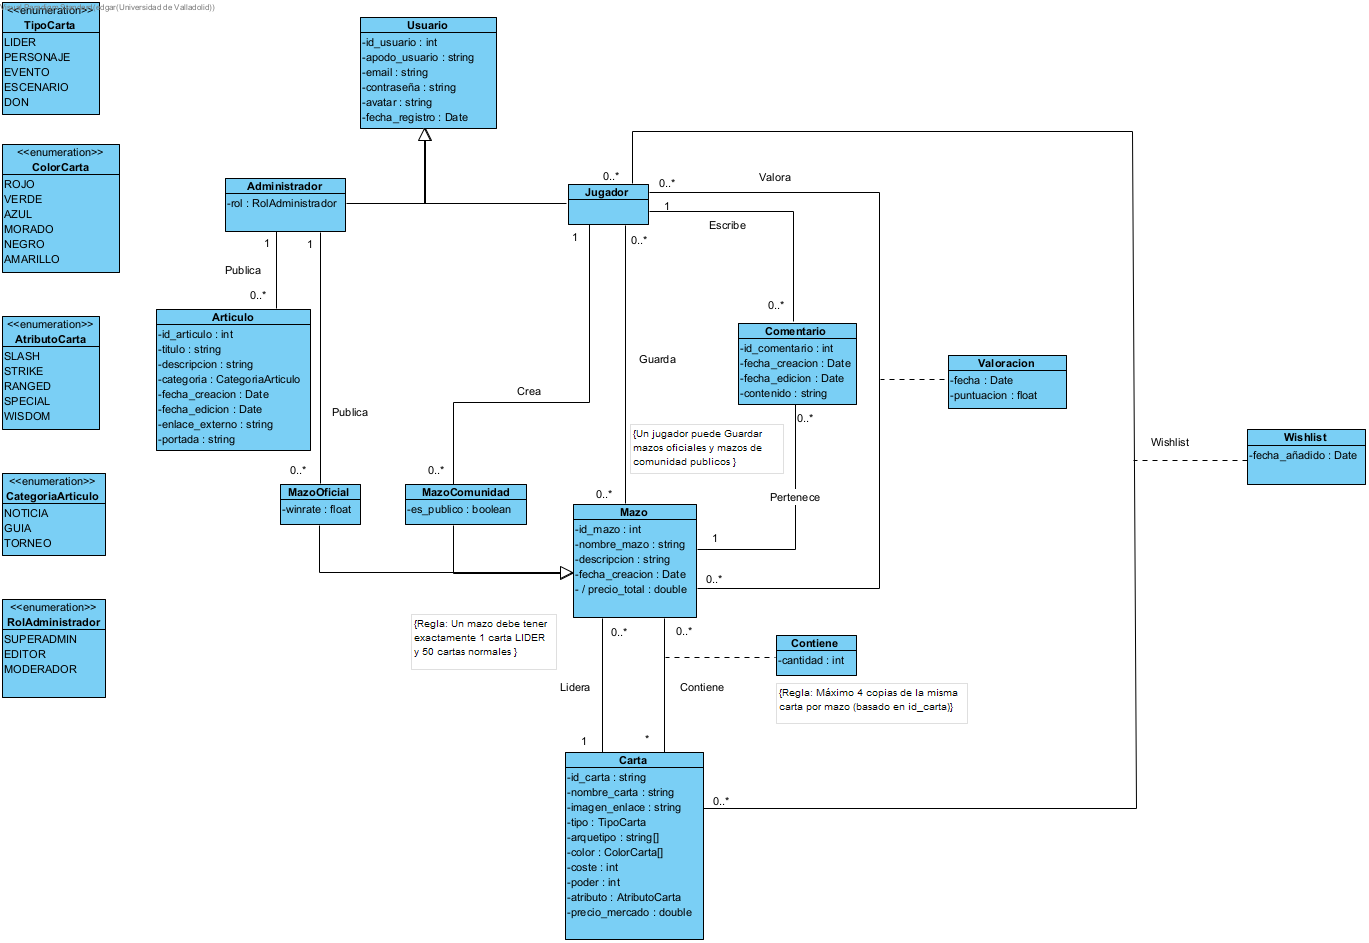
\includegraphics[width=0.9\textwidth]{Recursos/ModeloDominio_Grupo33.png}
		\caption{Diagrama UML del Modelo de Dominio de Card Partner}
		\label{fig:modelo_dominio}
	\end{figure}
	
	
	\newpage
	\section{Diseño del mapa del sitio web}
	El mapa del sitio web define la jerarquía de navegación y la reutilización de vistas y centralización de las herramientas. La estructura está diseñada para facilitar el acceso rápido a las diferentes herramientas de Card Partner a través de su menú de navegación en la barra superior de la página, disponible en cualquier momento.\\
	
	El mapa está estructurado en 4 niveles de profundidad para facilitar una entrada sencilla y estructurada a las herramientas:.\\
	\begin{itemize}
		\item \textbf{Nivel 0: Punto de entrada}\\
			El nivel 0 es la base de la estructura de la web, la \textbf{Página Principal} y es el punto de entrada de los usuarios. Desde ahí se muestra accesos rápidos a diferentes subsecciones de la web que pueden ser interesantes para usuarios nuevos o novedades para los usuarios experimentados.\\
		\item \textbf{Nivel 1: Navegación global}\\
			El nivel 1 es la base de la navegación dentro de la web. El \textbf{Menú principal} es la barra de navegación accesible en todo momento que divide la web en 4 grandes secciones, correspondientes al nivel 2 que son las herramientas para el usuario\\
		\item \textbf{Nivel 2: Herramientas y listados}\\
			El nivel 2 son las diferentes herramientas y visualización de contenido que ofrece la web a los usuarios, que se han dividido en 4 secciones:
			\begin{itemize}
				\item \textbf{SOCIAL:} Este apartado se divide en 3 subsecciones, el \textbf{Listado de Noticias}, \textbf{Listado de Torneos} y \textbf{Listado de Guías}. Funcionan de manera similar, mostrando en diferente formato los contenidos publicados, permitiendo acceder a ellos lo que les dirigirá a un visualizador con más información específica, siendo respectivamente el \textbf{Visualizador de Noticia}, el \textbf{Visualizador de Torneo} y el \textbf{Visualizador de Guia}
				\item \textbf{CARTAS:} Este apartado llevará directamente al \textbf{Listado de cartas}, página donde se mostrarán las cartas del TCG y se podrá acceder a cada una de ellas, dirigiendo al \textbf{Visualizador de carta} que mostrará más información en detalle sobre la carta seleccionada.
				\item \textbf{MAZOS:} Este apartado agrupa las herramientas referidas a los mazos; el \textbf{Creador de mazos} que es la herramienta que permitirá al usuario crear su propio mazo eligiendo las cartas de la web, y el \textbf{Listado de Mazos}, que desde esta sección se podrá acceder a 2 contenidos distintos, \textbf{Listado de mazos comunidad} que son los mazos creados y publicados por los usuarios de la web y \textbf{Listado mazos META}, que son los mazos más recomendados en la actualidad por toda la comunidad de TCG por sus estadísticas.
				\item \textbf{USUARIO:} El apartado usuario se divide en 2 secciones en función si el usuario ha iniciado sesión o no.\\
				Si no ha iniciado sesión, se podrá crear un nuevo usuario o iniciar sesión con una cuenta registrada, lo que devolverá al usuario a la página en la que se encontrase con las nuevas funcionalidades posibles con sesión iniciada.\\
				Con la sesión iniciada, se mostrarán las secciones de \textbf{Gestión de Mi Cuenta} y las secciones de \textbf{Gestión de Mis Mazos}, \textbf{Gestión de Mazos Publicados}, \textbf{Gestión de Mazos Guardados} y \textbf{Gestión de Mazos Vistos}, que redirigirá al \textbf{Listado de Mazos} con los diferentes contenidos respectivamente, y a su vez podrá redirigir al \textbf{Creador de mazos} para editar los mazos del usuario.
			\end{itemize}
			
		\item \textbf{Nivel 3: Visualizadores y detalle}\\
			El nivel 3 es el referido a los visualizadores mencionados que ofrecen el máximo detalle del contenido de la web, donde convergen los distintos listados de contenido del nivel 2.
	\end{itemize}
	
	\begin{figure}[H]
		\centering
		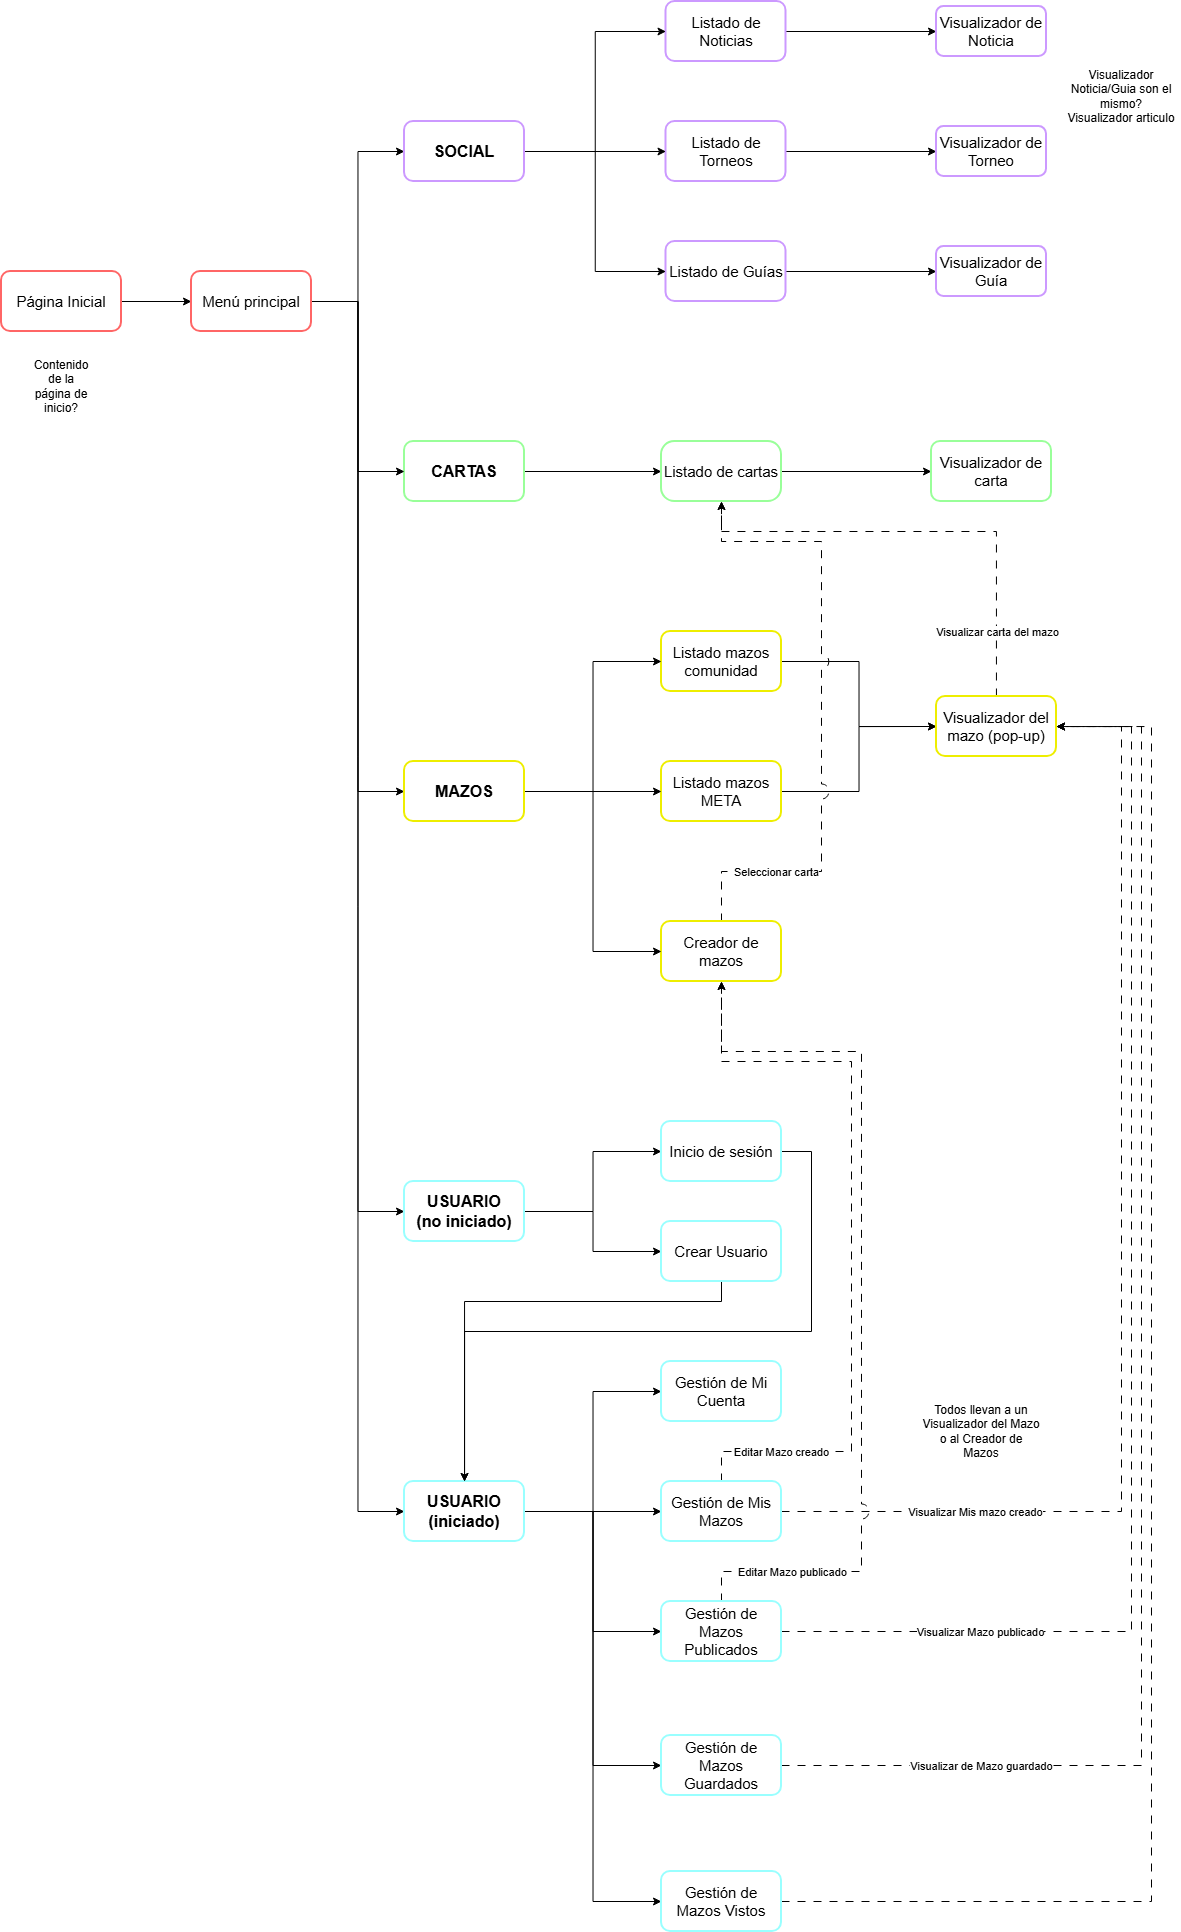
\includegraphics[width=0.9\textwidth]{Recursos/Mapa Card Partner v1.png}
		\caption{Estructura jerárquica y mapa del sitio web de Card Partner.}
		\label{fig:mapa_sitio}
	\end{figure}
	
	\subsection{Flujos de navegación}
		\subsubsection{Consulta de mazos}
		\subsubsection{Crear mazo}
		\subsubsection{Consultar noticias}
		\subsubsection{Consulta de cartas}
		
		
	
	\section{Cambios con respecto a la idea inicial}
		En este apartado comentaremos los cambios que hemos tenido con respecto a la idea incial
		\subsection{Torneos}
			Esta sección de la web estaba planteada para mostrar información de los torneo, esto supone, que un administrado tiene que estar mirando constantemente todos los torneos, ya sean locales, regionales o mundiales, para ir actualizando la vista de cada uno de ellos. \\ 
			Debido a la gran cantidad de los mismos, y  la dificultad para establecer un filtro de qué torneos en qué regiones son representativos hemos decidido aplicar un enfoque similar al apartado de notificas y de guías, tener enlaces a cada uno de los torneos, y para los winrates, tener esa información en el apartado de mazos meta, puesto que esta estadística, aporta una información mucho más útil de los mazos  de una manera más simple, permitiendo al usuario de un vistazo consultar qué mazos son META sin necesidad de tener que navegar por los diferentes torneos.
	\newpage
	\section{Reparto de carga de trabajo}
	Todos los integrantes hemos participado en todas las fases del trabajo y repartido el trabajo de forma equitativa, aunque encargándonos cada uno especialmente de alguna parte.\\
	
	\begin{table}[h]
		\centering
		\caption{Distribución de Responsabilidades por Miembro}
		\begin{tabularx}{\textwidth}{llX} 
			\toprule
			\textbf{Nombre} & \textbf{Porcentaje} & \textbf{Responsabilidad principal} \\
			\midrule
			ÁLVAREZ FULCONIS, MARCOS PALATINO      	& 25\%                & Diseño de las vistas tcg, social,noticias,torneo y guías\\
			LOPEZ PRIMO, ÁLVARO      				& 25\%                & Diseño del index, login y todas sus opciones, creación del repositorio de github, redacción del documento\\
			OTERO GARCÍA, SERGIO     				& 25\%                & Diseño de decks y todos sus submenús, \textit{comunity decks, meta decks}, creación de mazos,vista de cartas\\
			SANTIESTEBAN MENDO, EDGAR    			& 25\%                & Modelo de dominio,flujos de navegación, requisitos y redacción del documento\\
			\bottomrule
		\end{tabularx}
	\end{table}
	
	
	\section{Declaración de Uso de Inteligencia Artificial}
	Para esta primera entrega más creativa, se ha usado la IA \href{https://gemini.google.com/share/938828584764}{Gemini} como herramienta únicamente para mejorar la presentación del documento PDF. \\
	Principalmente se ha usado para dudas y mejoras del archivo LaTeX y para realizar una revisión rápida de ortografía y estructura del documento.\\
	
	\textbf{Ejemplos de prompts realizados:}
	\begin{itemize}
		\item 'Cómo podemos realizar un menú desplegable en html a partir de un botón'
		\item 'Cómo podemos hcer un enlace en una imagen'
		\item 'Cómo podemos hacer un popup para cambiar la contraseña'

	\end{itemize}
	
	%\begin{itemize}
	%   \item Herramientas utilizadas: hay que especificar qué herramientas de IA se han utilizado.
	%  \item Propósito del uso: explicar cómo se ha utilizado cada herramienta.
	% \item Alcance del uso: indicar en qué partes específicas del trabajo se ha recibido asistencia de una herramienta de IA.
	%\item Prompts utilizados: incluir los prompts, preguntas o instrucciones exactas que se han
	%introducido en la herramienta de IA.
	%\end{itemize}
	
\end{document}